% R. IMPORTANTE. In questa capitolo c'é anche la valutazione come sezione. Il capitolo é troppo ampio e ha un eccessivo accoppiamento. Dividerei. fatto, capitolo 5_evaluation
% \chapter{Ontology implementation}
\chapter{The Prompt Engineering Ontology: Implementation}
\label{chapter:4_implementation}
% R. Spiegazione modifica. Migliorata la scrittura.
% In this chapter I describe the actual implementation of prompt engineering ontology starting from functional and non-functional requirements defined in the previous chapter.
This chapter describes the implementation of PEO starting from the functional and non-functional requirements.
The LOT methodology includes four steps: 
\begin{enumerate}
    \item Ontology conceptualization

    \item Ontology reuse

    \item Ontology encoding

    \item Ontology evaluation
\end{enumerate}
% R. Spiegazione modifica. Le figure vanno referenziate. Evitare cose del tipo the figure below o : . Queste presuppongono che le figure siano sempre dopo il testo in cui le si commenta, ma questo é impossibile da prevedere. Con il riferimento la figura puó essere anche in testa alla pagina e il commento in mezzo al testo. Ho fatto diversi esempi di questa cosa nel capitolo 2.
% In the Fig. \ref{fig:14} the ontology implementation workflow according to LOT:

\begin{figure}[H]
    \centering
    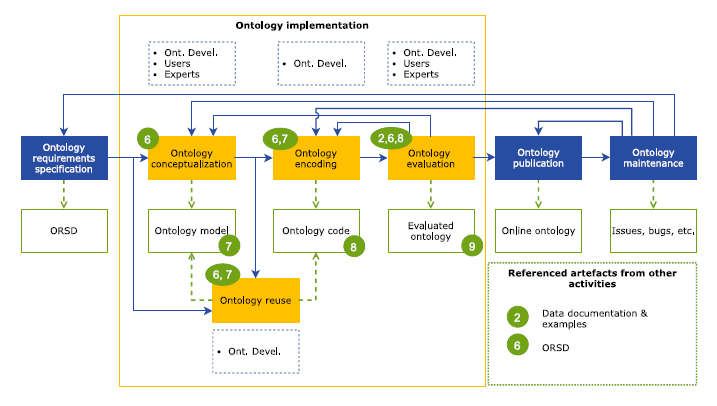
\includegraphics[width=0.9\linewidth]{Figures/fig_14.png}
    \caption{Ontology implementation workflow}
    \label{fig:14}
\end{figure}
Fig. \ref{fig:14} represents the ontology implementation workflow according to LOT.
At the end of this phase, the output is an ontology ready to be published and to be made available online.

% \newpage
% \section{Ontology Conceptualization}
\section{Conceptualization}
\label{section:4_1_conceptualization}
The first step in the ontology implementation is the ontology conceptualization, we define of all main concepts in the ontology with the relations among them.
% R. Richiesta modifica. Evitare 'I'. Non metteró piú il commento. fatto
We used \href{draw.io}{https://app.diagrams.net/} software: a free easy-to-use diagramming tool that allows to represent UML diagrams and many more.
% R. Richiesta modifica. Usare la punteggiatura e dividere la frase prima di moreover. Togliere '\\'. Per l'ultima cosa non metteró piú il commento. 
We chose this software over other diagramming tools because it is intuitive, easy to use, and frequently updated moreover with draw.io. It is possible to export diagrams in other formats like: svg, pdf and png in high resolution.
Starting from the CQs, we chose a top-down strategy in order to model the domain of prompt engineering and LLMs, modelling first major concepts and then going more into detail.
% R. Richiesta modifica. La domanda messa cosí confonde. Scrivere come affermazione o se vuoi lasciarla va posta meglio. Poi va chiarito che si intende con uesful e meaningful. Potresti provare a collegarti agli use case che hai definito per spiegare perché modelli certe cose piuttosto che altre. ho rimosso
% R. Richiesta modifica. Linguaggio troppo personale ("dwell too much") che non va bene, la tesi deve essere limitata a fatti e motivazioni. Motivazione vaga (magari sapere che un LLM é decoder only é una sottigliezza per un utente che vuole usare un LLM per scrivere una mail, ma non lo é per un ricercatore che vuole trovare il miglior LLM per il suo task e le sue risorse a disposizione). Se ti colleghi agli obiettivi e agli use cases eviti di cadere in opinioni personali (e discutibili). rimosso
A LLM is represented using four dimensions:
\begin{enumerate}
    % R. Richiesta modifica. la prima parte della frase non é chiara: sub concept di cosa?
    \item \textbf{Type:} type of LLM which is a sub concept. Each type of LLM has one or more instances representing versions of that LLM.

    \item \textbf{Organization:} organization that creates the LLM.

    % R. Richiesta modifica. Meglio attribute di characteristic. vedere anche altre occorrenze. fatto
    \item \textbf{Base model:} the deep learning model at the base of the architecture of the LLM. This concept represents an attribute of a LLM.

    \item \textbf{Capability:} the capability of a LLM, it is represents an attribute of a LLM.
\end{enumerate}
These concepts provide a representation of various aspects of LLMs, from their underlying architecture to the organizations that develop them, which can range from universities and research institutions to companies with business-oriented goals.
% R. Richiesta modifica. Usare gli acronimi, non scriveró piú il commento.
A fundamental aspect is the representation of the capabilities of LLMs.
In fact, the ontology will not only include LLMs capable of processing text but also multimodal models capable of handling more complex data types, such as images, audio, video, and source code.\\
Regarding prompt engineering, starting from the user's perspective, we decided to model the domain using the following concepts:
\begin{itemize}
    % R. Spiegazione modifica. Ripetizioni superglue all'inizio di ogni punto. Errore ripetuto per tutti gli elenchi puntati. Controllare tutte le occorrenze. Non scriveró piú il commento. era la ripetizione del nome? chiaro
    % \item \textbf{Prompting technique:} this concept gathers all the prompting techniques, each prompting technique is a sub concept.
    \item \textbf{Prompting technique:} gathers all the prompting techniques, each prompting technique is a sub concept.

    % R. Richiesta modifica. Qui pare che nel concetto prompt sia memorizzata anche la risposta. Se non é cosí togliere "followed by a response" che crea in confusione. Se invece é cosí dirlo esplicitamente per togliere ogni dubbio.
    \item \textbf{Prompt:} this is the base concept, a single prompt provided as input in the context of a chat with a specific LLM, followed by a response. The prompt can be generated using a prompting technique.

    \item \textbf{Chat:} represents the context of a prompt with a specific LLM and it can include one or more prompts and responses.

    \item \textbf{Response:} represents the response generated by LLM after the input of a prompt in the context of a specific chat.
\end{itemize}


In addition, there is also the modelling of the concept \textbf{"Task"} that represents the tasks to be solved using LLMs by applying prompting techniques.
This concept has sub concepts specific for the task that has to be solved like: image task, text task, code task, audio task and video tasks, each one of those concepts has other sub concepts, e.g., the "text task" has as sub concepts text summarization, emotion classification, text translation.

The concepts of \textbf{"Chat"} and \textbf{"Prompt"} are introduced to decouple each prompting technique from a specific LLM, ensuring their independence.
% R. Spiegazione modifica. Sostituito reasoning con intuition per evitare confusione con il reasoning nelle ontologie. Un termine deve rapprentare un unico concetto. E un concetto deve essere rappresentato da un unico termine. Altrimenti ci perdiamo in omonimi e sinonimi e diventa tutto piú ambiguo.
% The reasoning behind this conceptualization is simple and straightforward: a prompt is created using a specific prompting technique and applied in the context of a specific chat with a version of LLM producing a response.
The intuition behind this conceptualization is that a prompt is created using a specific prompting technique and applied in the context of a specific chat with a version of LLM producing a response.

% R. Richiesta modifica. Consistenza nello stile dei nomi delle classi.
The connection with the concept of Task lies in solving a specific task through the use of an instance of a prompting technique.
% R. Richiesta modifica. Le relations le hai definite come roles nel capitolo 2. Usare sempre lo stesso termine.
Once defined the major concepts in the ontology, we define the relations between these concepts.
Starting from the LLM, each sub concept like GPT, Mistral, Gemini is involved in the following relations:
% R. Richiesta modifica. Separare le parole nei nomi delle relazioni con '_'. Per esempio, has architecture -> has_architecture.
\begin{itemize}
    \item \textit{develops:} an organization develops a LLM type, for example Google develops Gemini.

    \item \textit{has architecture:} a LLM type has an architecture based on a specific base model. For example GPT has architecture the decoder-only model.
    
    \item \textit{has capability:} a LLM type is connected to a specific capability.
\end{itemize}
As we have seen, the aspect of different versions of the same model must be considered and appropriately represented.
To achieve this, we have used two distinct relations:
\begin{itemize}
    \item \textit{has variant:} this relation represents a contemporaneity between two models, where a model $x$ is a variant of a model $y$, and this does not represent an evolution of model $x$. For example Mistral-7B has variant Codestral (a version of Mistral specific for source code processing.)

    \item \textit{evolves:} unlike \textit{has variant}, this relation represents a temporal succession between an older model and a newer model, for example GPT-3 evolves GPT-4, where GPT-4 is a more recent and powerful version of GPT. For this relation, we have introduced also the inverse relation \textit{evolved from}.
\end{itemize}
Another specific aspect considered is the presence of relations between organizations developing LLMs, where one organization is part of another organization, for example, DeepMind is a research organization and is part of Google.
% R. Nota. Qui bisogna fare attenzione (per esempio se ne parli nella presentazione) perché facilmente scatta la domanda sul riuso. Ontologie sull'organizzazione industriale sicuramente ce ne sono.
We created two relations called: \textit{has organization} and \textit{is organization of} in order to represent this aspect in the ontology.
\begin{figure}[H]
    \centering
    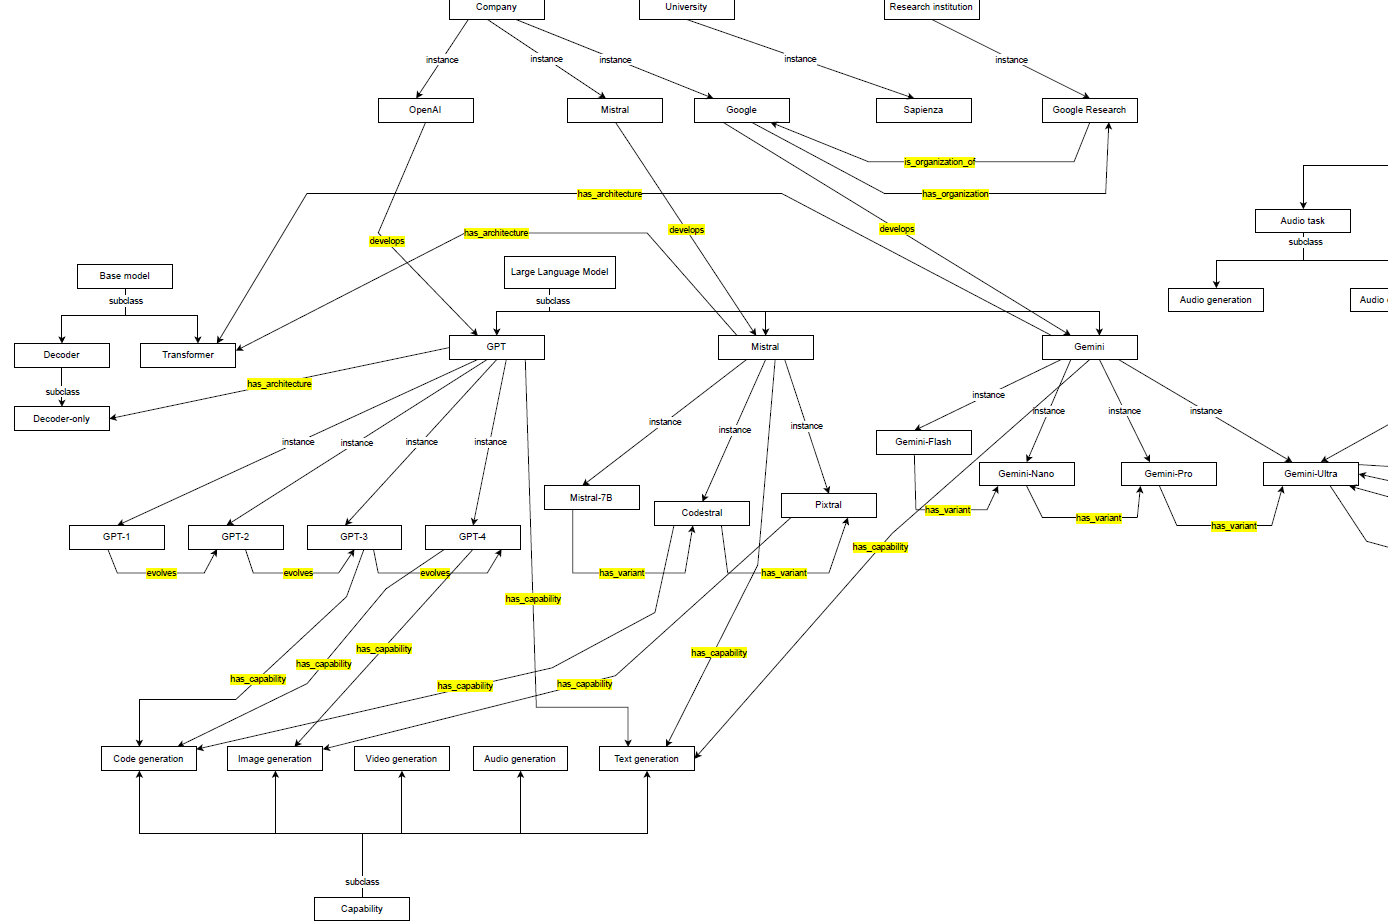
\includegraphics[width=0.9\linewidth]{Figures/fig_26.png}
    \caption{LLMs dimensions conceptualization}
    \label{fig:26}
\end{figure}
The Fig. \ref{fig:26} shows the conceptualization scheme for LLMs.

Regarding the prompt domain, the following relations have been created in order to properly connect the introduced concepts:

\begin{itemize}
    % \item \textit{solves task:} connects an instance of a prompting technique with an instance of a task, where the instance of the prompting technique solves that specific task. The inverse relation is: \textit{solved by}.
    \item \textit{solves task:} connects a prompting technique with a task. The inverse relation is: \textit{solved by}.

    \item \textit{is used in prompt:} connects a prompting technique with a prompt. The inverse relation is: \textit{prompt generated using}.

    \item \textit{has context:} connects a prompt with its context, i.e., a chat where such prompt and possibly more are connected to. The inverse relation is: \textit{has prompt}.

    \item \textit{uses model:} connects a chat with a LLM that is used to input prompts and generate responses. The inverse relation is: \textit{is used in chat}.

    \item \textit{generates response:} connects a LLM with the response generated after a prompt to such LLM. The inverse relation is: \textit{response generated using}.

    \item \textit{prompt follows response:} connects a prompt with its response, the inverse relation is: \textit{response followed by prompt}.

    \item \textit{has response:} connects a chat with a response, the inverse relation is: \textit{is response of}.
\end{itemize}
% R. Spiegazione modifica. Rimosso perché basta quella sotto la figura.
% The conceptualization of prompt engineering domain is represented.

\begin{figure}[H]
    \centering
    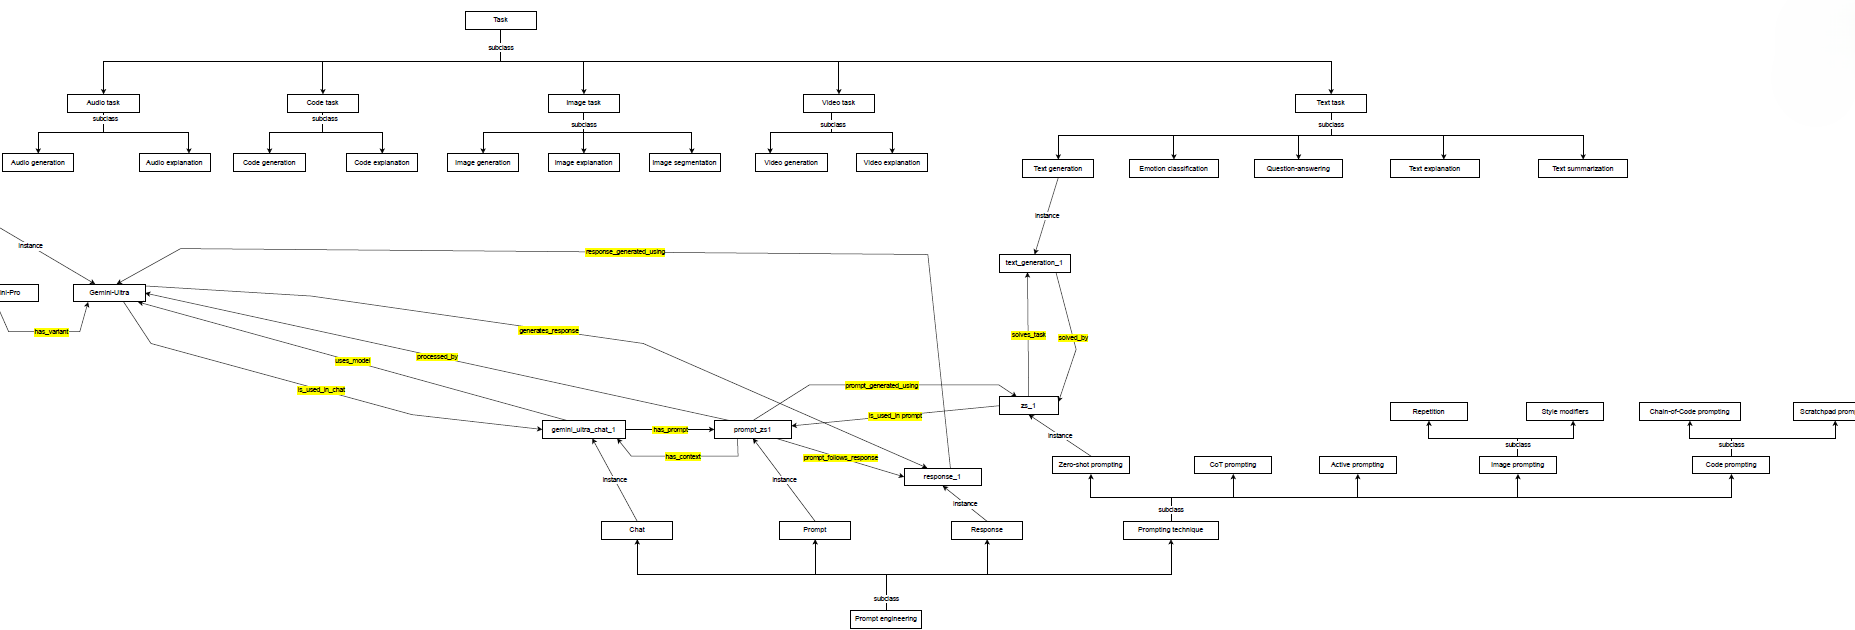
\includegraphics[width=0.9\linewidth]{Figures/fig_27.png}
    \caption{Prompt engineering\\ dimensions conceptualization}
    \label{fig:27}
\end{figure}
The Fig. \ref{fig:27} shows the conceptualization for Prompt Engineering part.

After completing the conceptualization phase, the process can proceed to ontology reuse and ontology encoding.
This involves first identifying similar ontologies within the domain of interest for potential reuse, followed by implementing and encoding the defined concepts using dedicated software tools.

\section{Reuse}
\label{section:4_2_reuse}
Before proceeding with ontology encoding, it is necessary to consider any similar ontologies that can be reused in the creation of the prompt engineering ontology. There are two types of reuse:
\begin{itemize}
    \item \textbf{Hard reuse:} involves directly importing an entire ontology, rigidly incorporating it. Classes and properties are used without modification, ensuring semantic consistency but creating strong dependency on the original ontology.

    \item \textbf{Soft reuse:} involves adapting or copying specific concepts without importing the complete ontology. This approach offers more flexibility, allowing customization, but it may introduce semantic inconsistencies or redundancies 
\end{itemize}

\subsection{Ontology Design Patterns Reuse}
\label{subsection:4_2_1_design_patterns}
During the design of PEO, we decided to use three design patterns:
\begin{itemize}
    \item \textbf{Description pattern}
    \item \textbf{Sequence pattern}
    \item \textbf{Task Execution}
\end{itemize}
% R. Spiegazione modifica. Rimosso: é un concetto basic (detto nel capitolo 2). Questo é il capitolo dove si capisce cosa hai fatto tu.
% those design patterns are useful to represent better concepts in the ontology without inventing anything from zero.

The description pattern is used in the definition of subclasses of \textit{LLM} class, where its subclasses describe the LLM class.\cite{description_pattern}
In fact, this ODP allows the designer to represent both a (descriptive) context and the elements that characterize and are involved in that context.

\begin{figure}[H]
    \centering
    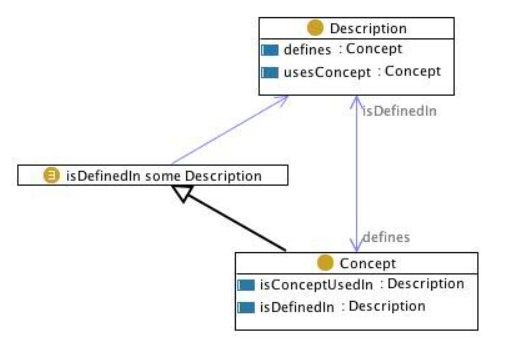
\includegraphics[width=0.6\linewidth]{Figures/fig_73.png}
    \caption{Description pattern}
    \label{fig:73}
\end{figure}
The Fig. \ref{fig:73} shows graphically the Description pattern.

%% R. Richiesta modifica. "this"? Sequence pattern
The sequence pattern is used in the ontology to represent evolutionary aspects, specifically among instances of LLMs, involving the relationships \textit{evolves} and \textit{evolves\_from}.
This ontology design pattern allows to represent and reason over transitive or intransitive sequences of any kind \cite{sequence_pattern}.
\begin{figure}[H]
    \centering
    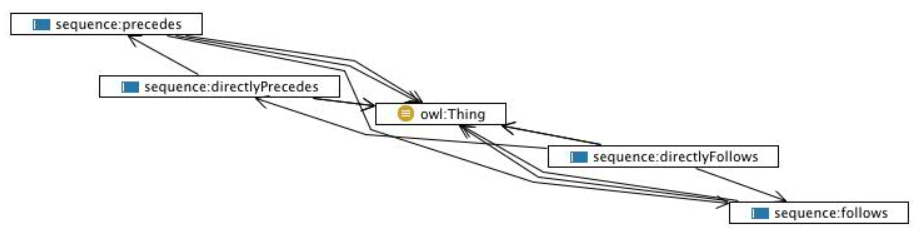
\includegraphics[width=0.8\linewidth]{Figures/fig_74.png}
    \caption{Sequence pattern}
    \label{fig:74}
\end{figure}
The Fig. \ref{fig:74} shows graphically the Sequence pattern.

% R. Richiesta modifica. "This" quale? fatto
The task execution pattern is partially used in the representation of task instances executed (solved) by an instance of a prompting technique. More in general, this ODP allows designers to make assertions on roles played by agents without involving the agents that play that roles, and vice versa\cite{task_execution}.

\begin{figure}[H]
    \centering
    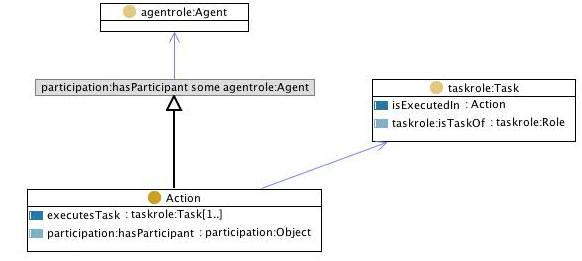
\includegraphics[width=0.8\linewidth]{Figures/fig_75.png}
    \caption{Task Execution}
    \label{fig:75}
\end{figure}
The Fig. \ref{fig:75} shows graphically the Task Execution pattern.

\subsection{State-of-the-art Ontologies Reuse}
\label{subsection:4_2_2_reuse}

I considered two ontologies that can be reused for the implementation of prompt engineering ontology:
\begin{enumerate}
    \item HALO ontology

    \item AI ontology
\end{enumerate}


The HALO ontology \cite{nananukul2024halo}, reviewed in the state-of-the-art chapter, has been considered due to its relevance to a domain closely connected to LLMs, specifically addressing the hallucinations they generate.
The ontology is accessible on GitHub \footnote{https://github.com/navapatn/halo-ontology}.
% R. Spiegazione modifica. Non ci interessa molto del paper, stiamo parlando di ontologie. Linguaggio troppo personale.
% Despite, the complete and exhaustive paper published, the published ontology is very poor.
However, we decide not to reuse it.
This is because it is mostly focused on the hallucinations rather than LLMs and prompts themselves (our target).
Indeed, the class hierarchy on LLMs is shallow in favour of a deeper one on hallucinations.
As such, we deemed the reuse more effortful than the implementation from based on the outcomes of the previous phases that we executed focusing on our target rather than hallucination.


% R. Nota. Motivazioni precedentemente esposte da Simone. Non mi sembravano convincente. Lasciate commentate.
% It has just twenty-five classes and none of them has an annotation or something to explain better the concept.
% R. Richiesta modifica. E perché é un difetto il fatto che abbia una gerarchia di classi sulle allucinazioni?
% There is a class called \textit{"LLMs Hallucination"} with two subclasses called \textit{"factuality hallucination"} and \textit{"faithfulness hallucination"}. Each one has subclasses about the type of hallucination that represent.
% R. Perché sono inutili queste classi? Provo a spiegare: verificare.
% Moreover, there are pretty useless classes like \textit{"answers"} or \textit{"Book"} that seem have no sense in an ontology of this type, there are no individuals and just nine unused object properties.
% R. Anche questa non impedisce il riuso: basta toglierle. Se non creano inconsistenze o altro.
% Moreover, there are disconnected and not instantiated classes like \textit{"answers"} or \textit{"Book"}.
% R. Se non ci sono indiviui é impossibile che le relazioni siano usate in delle triple, il problema quindi é che é vuota e l'abbiamo giá detto. Piuttosto, le relazioni hanno domain e range? Si sa se sono transitive/riflessive/simmetriche/... ? solo domain e range sta e basta. R. non é poco. Tutte queste motivazioni ti danno la zappa sui piedi
%In addition, object properties .
% This was sufficient to conclude that the HALO ontology would not be reused in the development of PEO, as it would not offer any meaningful or valuable information.\\

% The second ontology took into account is the Artificial Intelligence Ontology\cite{aio}, an ontology that covers machine learning methods, deep learning networks and their components.
The second ontology considered for reuse is the Artificial Intelligence Ontology \cite{aio}, an ontology that covers machine learning methods, deep learning networks and their components.
This ontology is particularly intriguing, as it stands out as one of the few, if not the only, ontologies focused on the field of artificial intelligence.
% R. Spiegazione modifica. Usare i pronomi per evitare le ripetizioni (senza esagerare) (esempio qui it al posto di this ontology).
It is available on its GitHub repository \footnote{https://github.com/berkeleybop/artificial-intelligence-ontology} in OWL, json and csv format. 

% R. Richiesta modifica. Verificare e sistemare (scritto bveloce).
However, we decide not to reuse it, this is because, it mostly is a class hierarchies, while lacking roles.
Moreover, it is focused on machine learning methods.
As such, with the goal of obtaining a broader ontology, it can be seen of an upper level in the hierarchy of LLMs in PEO.
In contrast, PEO describes in more detail LLMs through lower levels in the hierarchy and relationships with the other concepts specific to domain of PEO.




\section{Encoding}
\label{section:4_3_encoding}
% \subsection{Software in ontology encoding and the Protégé editor}
\subsection{Software and Tools}
\label{subsection:4_3_1_software}
The ontology encoding phase is where the ontology is actually implemented.
% R. Richiesta modifica. Aggiungere quale linguaggio abbiamo scelto noi (e perché).
During this stage, the concepts and relationships defined in the conceptualization phase are formalized in OWL. We choose it because it is the standard in the semantic web and it allows to represent complex knowledge by using classes, object properties, data properties, individuals and annotations.

Several tools are available to assist developers with this task.
The main software tools for implementing ontologies include:
\begin{itemize}
    \item Protégé \footnote{https://protege.stanford.edu/}
    \item FluentEditor \footnote{https://www.cognitum.eu/semantics/fluenteditor/}
    \item Vitro \footnote{https://github.com/vivo-project/Vitro?tab=readme-ov-file}
    \item OntoStudio \footnote{https://www.semafora-systems.com/ontobroker-and-ontostudio-x}
\end{itemize}
% R. Richiesta modifica. Evitare "my project". In generale usare forme impersonali o al limite "we". ok
To begin, we chose Protégé: an open-source ontology editor developed by a team at Stanford University since 1987.
Widely used and highly regarded among ontology engineers, it offers a user-friendly Eclipse-based interface and a wide range of features.
% R. Richiesta modifica. Digressione troppo lunga. Togliere la lista delle features o delegare al capitolo 2. tolta

Only a limited number of ontology editors provide an extensive set of features tailored for developers.
Moreover, several editors have remained outdated for years and suffer from lots of bugs.
During the ontology development process, \href{https://git-scm.com/}{Git} was also used: a version control software to track changes made to the ontology that are synchronized with the GitHub repository \footnote{https://github.com/simonegramegna/peo}.

% R. Spiegazione modifica. Evitare gli acronimi nei titoli.
% R. Richiesta modifica. Cosa intendi con encoding beginning?
% \subsection{Encoding beginning PEO}
% \subsection{Encoding beginning Prompt Engineering Ontology}
\subsection{First Steps}
\label{subsection:4_3_2_encoding}
% R. Richiesta modifica. Correggere la definizione dell'acronimo. fatto. R. non mi sembra, vedo la versione per intero tra parentesi, é il contrario. Inoltre, probabilmente é giá stato definito questo acronimo, quindi ti basta usarlo.
Starting from an empty page, the first thing to do is the definition of the ontology IRI (Internationalized Resource Identifier): which has to be unique and it has to refer to a standard organization.
The ontology IRI of the PEO is: \textit{https://w3id.org/peo\#}; this IRI will be in every entity created inside the ontology.
\begin{figure}[H]
    \centering
    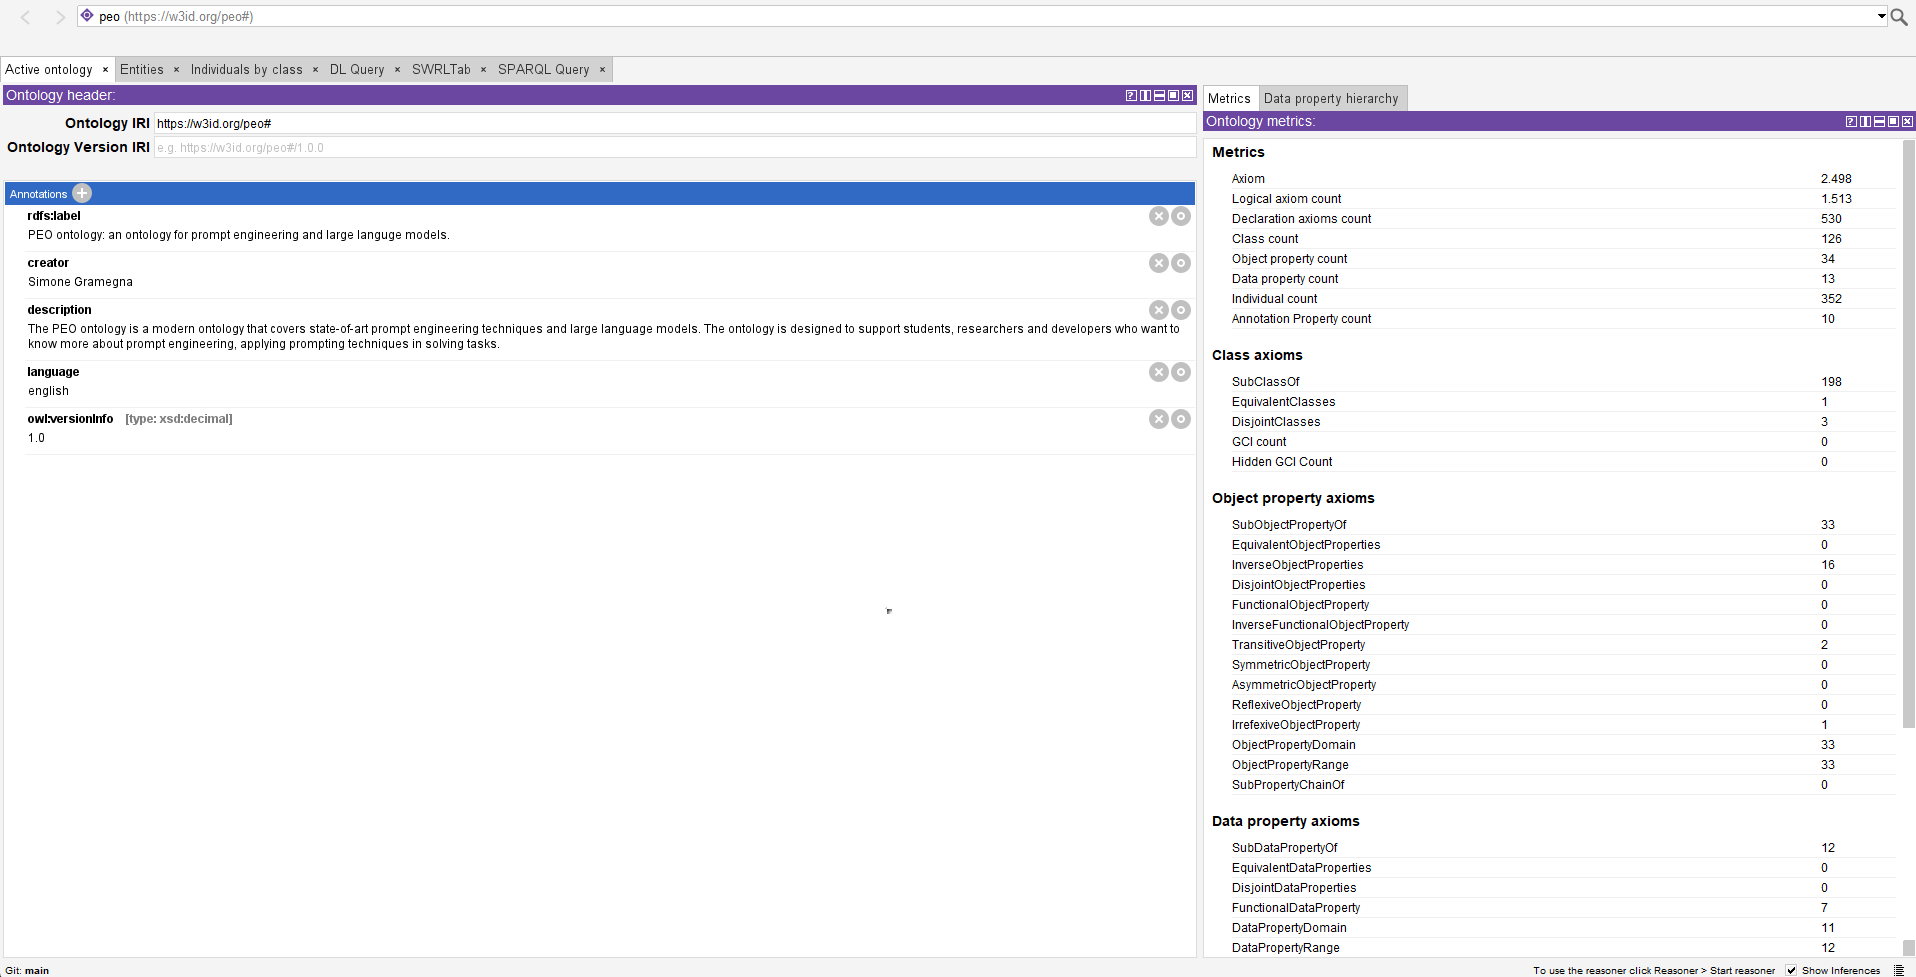
\includegraphics[width=0.8\linewidth]{Figures/fig_29.png}
    \caption{PEO main page}
    \label{fig:29}
\end{figure}
% R. Spiegazione modifica. Fig. é terza persona singolare. Errore ripetuto.
Fig. \ref{fig:29} shows the PEO main page.
% R. spiegazione modifica. semplificato.
% R. Nota. Le label a tabelle e figure si mettono per far si che quando cambi il loro ordine hai comunque una lable identificativa che prescinde dell'ordine. Quindi, serve a poco deifnire le label per tabelle e figure se nelle label metti l'ordine in cui compaiono. Se cambia l'ordine delle tabelle devi anche cambiare le label.
Once created the IRI, we define the five annotations and we report them in Tab. \ref{table:t_4_1}. % to properly describe the ontology:
\begin{table}[H]
    \centering
    \begin{tabular}{|>{\raggedright\arraybackslash}p{6cm}|>{\raggedright\arraybackslash}p{6cm}|}
        \hline
        \textbf{Annotation} & \textbf{Annotation value} \\ \hline
         rdfs:label & PEO: an ontology for prompt 
         engineering and LLMs. \\ \hline
         
         creator & Simone Gramegna\\ \hline
         
         rdfs:comment & The PEO is a modern ontology that covers state-of-art prompt engineering techniques and LLMs. The ontology is designed to support students, researchers and developers who want to know more about prompt engineering, applying prompting techniques in solving tasks. \\ \hline
         
         language & English \\ \hline
         
         owl:versionInfo & 1.0 \\ \hline
    \end{tabular}
    \caption{Ontology annotations in the main page}
    \label{table:t_4_1}
\end{table}


Starting from the concepts outlined in the conceptualization phase, we define the primary classes of the ontology, which include:
\begin{itemize}
    \item \textbf{Base model}

    \item \textbf{Capability}

    \item \textbf{Large Language Model}

    \item \textbf{Organization}

    \item \textbf{Prompt engineering}

    \item \textbf{Task}
\end{itemize}
All these classes are mutually disjoint, as they represent distinct entities with no overlapping properties.
% The only exception is the relationship between "Base model" and "Capability", which are not disjoint.
The only exception is given by "Base model" and "Capability", which are not disjoint.
Both represent attributes of LLMs and are collectively grouped under the \textbf{"LLM characteristic"} class, formed by the union of the two classes. \\
The Capability has five subclasses, each subclass has a label and a comment:
\begin{table}[H]
    \centering
    \begin{tabular}{|>{\raggedright\arraybackslash}p{6cm}|>{\raggedright\arraybackslash}p{6cm}|}
        \hline
        \textbf{Label} & \textbf{Comment} \\ \hline
         Audio processing &  Capability to process audio files. \\ \hline
         
         Code processing & Capability to process source code written in any programming language. \\ \hline
         
         Image processing & Capability to process images, understanding the content of the image. \\ \hline
         
         Text processing & Capability to process text and documents with text inside. \\ \hline
         
         Video processing & Capability to process video files. \\ \hline
    \end{tabular}
    \caption{Capability subclasses}
\end{table}
Each subclass has an individual with the same name, those individuals are created with the aim of assigning a capability to the instances of LLMs that possess it, this aspect will be discussed later.

\subsection{Definition of Large Language Models and their Characteristics}
\label{subsection:4_3_3_llms}
The class "Base model" represents the models at the base of the architecture of LLMs, it has six subclasses each one with label, description and reference.
A subclass can have another subclass representing a more specific architecture, for example the subclass "Decoder" has the subclasses "Decoder only" and "Pixel decoder". 
I have included only the foundational models of the LLMs represented in the ontology, excluding other base models as they fall outside the scope of this ontology.
The subclasses included are: 
\begin{table}[H]
    \centering
    \begin{tabular}{|>{\raggedright\arraybackslash}p{6cm}|>{\raggedright\arraybackslash}p{6cm}|}
        \hline
        \textbf{Class} & \textbf{Subclasses} \\ \hline
         CLIP & none \\ \hline
         
         Decoder & Decoder-only, Pixel decoder \\ \hline
         
         Diffusion model & none \\ \hline
         
         Encoder & Encoder only, Global Image Encoder, Grounding Image Encoder, Region Encoder, ViT Encoder \\ \hline
         
         Recurrent Neural Network & none \\ \hline

        Transformer & Q-Former, LAMDA PT, Transformer XL \\ \hline
    \end{tabular}
    \caption{Base model subclasses}
\end{table}
The class "LLM characteristic" is a subclass of both "Base model" and "Capability".
Each LLM subclass is connected to those two classes using the relations: \textit{has\_capability} (inverse relation \textit{is\_capability}) and \textit{has\_model\_architecture}.
In total there are 33 LLMs subclasses of LLM, each representing a type of LLM such as GPT, Gemini ecc.
The definition of LLMs is completed with a label, a description, a link to the paper, and a link to the website.
Below there are LLMs in PEO with their capabilities and architecture.

% R. Spiegazione modifica. Unite le due parti della tabella. 
\begin{table}[H]
    % \small
    \footnotesize % ridotto font
    % ancora piú piccoli
    % \scriptsize
    % \tiny
    \centering
    \begin{tabular}{|>{\raggedright\arraybackslash}p{4cm}|>{\raggedright\arraybackslash}p{4cm}|>{\raggedright\arraybackslash}p{4cm}|}
        \hline
        \textbf{LLM} & \textbf{Capabilities} & \textbf{Base models} \\ \hline
        Alpaca & Text processing & Transformer\\ \hline
        BERT & Text processing & Encoder only \\ \hline
        BLIP-2 & Image processing & Q-Former \\ \hline
        BLOOM & Text processing & Transformer \\ \hline
        Chinchilla & Text processing & Transformer \\ \hline
        Claude & Text processing & Transformer \\ \hline
        CogVLM & Image processing & ViT Encoder \\ \hline
        Command R & Text processing & Transformer \\ \hline
        DALL-E & Image processing & CLIP, Decoder, Transformer \\ \hline
        Falcon & Text processing & Decoder only \\ \hline
        FLAN & Text processing & LAMDA PT \\ \hline
        Gemini & Audio processing, Code processing, Image Processing, Text processing, Video processing & Transformer\\ \hline
        Gemma & Text processing & Transformer \\ \hline
        GLaMM & Image processing & Global Image Encoder, Grounding Image Encoder \\ \hline
        LLaMA & Text processing & Transformer \\ \hline
        Midjourney & Image processing & Diffusion model  \\ \hline
        Minerva & Text processing & Transformer \\ \hline
        Mistral & Text processing & Transformer \\ \hline
        MPT-7B & Text processing & Decoder only \\ \hline
        OLMo & Text processing & Decoder only \\ \hline
        OpenELM & Text processing & Decoder only \\ \hline
        OPT & Text processing & Transformer \\ \hline
        PaLM & Text processing, Code processing & Transformer \\ \hline
        Phi-1 & Text processing & Transformer \\ \hline
        RWKV LLM & Text processing & Recurrent Neural Network, Transformer \\ \hline
        Sora & Video processing & Decoder only \\ \hline
        StableLM & Text processing & Decoder only \\ \hline
        StarCoder & Code processing & Decoder only \\ \hline
        T5 & Text processing & Transformer \\ \hline
        VALL-E & Audio processing & Transformer \\ \hline
        Vicuna & Text processing & Transformer \\ \hline
        XLNet & Text processing & Transformer XL \\ \hline
    \end{tabular}
    \caption{Large language models in PEO}
\end{table}
There is a relation \textit{based\_on} between two subclasses of LLM (with inverse relation \textit{basis\_for}) where a LLM is developed starting from the base of another LLM.
For example Alpaca is based on LLaMA (another family of LLMs).
Each type of LLM has a capability, this capability is common for all instances of the LLM.
Hence, if a specific version of a LLM has a new capability, the single LLM can be connected to that specific capability. For example, GPT has capability text processing but GPT-3.5 has also the capability of code processing so this version has two capabilities (text processing and code processing).
Same goes for GPT-4 which is an evolution of GPT-3.5 and has also the image processing capability; so it has three capabilities (text processing, code, processing and image processing).
This approach is very flexible because there is no need to divide into categorical classes each version of LLM by simply connecting the version with the specific instance of the capability.
There are three relations between versions of the same LLM: 
\begin{itemize}
    \item \textit{has\_variant:} relation between two LLMs (x and y), where x has y as another version.

    \item \textit{evolves:} transitive relation between two LLMs (x and y), where y is an evolution of x. 

    \item \textit{evolved\_from:} transitive inverse relation of \textit{evolves} between two LLMs x and y.
\end{itemize}

% R. Richiesta modifica. Frase ingarbugliata, rendere piú chiara (prendi ad esempio le modifiche che ho fatto). Specificare che usi SWRL perché vuoi fare un'inferenza. Per il momento omettiamo il perché é fatta in SWRL l'inferenza perché é venuto fuori che non ce n'era motivazione.

The relation \textit{has\_variant} express a different version of the model, while the relation \textit{evolves} specifies the evolution between two LLMs. 
The latter can also be used to infer the former.
For example, if GPT-3.5 evolves GPT-4 then GPT-3.5 has variant GPT-4.
We use SWRL rules to infer this connection. 
The chosen reasoner is the Hermit reasoner\cite{glimm2014hermit}: a reasoner already included in Protégé which does not require the installation of any additional plug-in.
The reasoner ensures the ontology consistency, inferring new axioms and processing SWRL rules.

SWRL rules are widely applied in PEO.
% R. Spiegazione modifica. semplificato e reso piú cjharo.
% the first application is the creation of a new relation \textit{has\_variant} if there is the \textit{evolves} relation, the rule is expressed in this way:
Firstly, they can infer the relation has\_variant from the relation  \textit{evolves}. Specifically, the rule is:
\begin{lstlisting}
peo:evolves(?x, ?y) -> peo:has_variant(?x, ?y)
\end{lstlisting}
$?x$ and $?y$ are the two instances involved in the relations.
The rule is applied to all instances that satisfy the condition in the body of the rule.
If a model evolves into another model, the evolved model has the capabilities of the previous model.
This concept is expressed using this SWRL rule:
\begin{lstlisting}
peo:evolves(?x, ?y) ^ peo:has_capability(?x, ?c) -> peo:has_capability(?y, ?c)
\end{lstlisting}
These two relations are not explicitly defined in the ontology, but are inferred by the reasoner. % R. rimosso. during the reasoning process, making them visible at that stage.
Each instance of the LLM has two data properties associated 
\begin{itemize}
    \item \textit{has\_number\_parameters:} number of parameters of the model.

    \item \textit{has\_release\_year:} year of release of the model
\end{itemize}
Those two data properties are functional, assigning a single value of each property to the instance of the LLM.

Large language models are developed by organizations that can be universities, research institutions and companies for business purpose, the class \textbf{Organization} contains has such three subclasses (with label  and description).
% Spiegaizone modifica. R. Rimosso. Non c'é bisogno di specificarlo smepre. Le classi le creiamo per istanziarle poi.
%and each subclass has instances representing the specific organization. chiaro
\begin{table}[H]
    \centering
    \begin{tabular}{|>{\raggedright\arraybackslash}p{6cm}|>{\raggedright\arraybackslash}p{6cm}|}
        \hline
        \textbf{Subclass or organization} & \textbf{Number of entities} \\ \hline
        
        University & 2 \\ \hline
 
        Research institution & 8 \\ \hline
        
        Company & 13 \\ \hline
    \end{tabular}
    \caption{Number of organization entities}
\end{table}
Every instance of organization has two associated data properties:
\begin{itemize}
    \item \textit{registered\_name:} the official name of the organization.

    \item \textit{official\_website:} the official website of the organization.
\end{itemize}
Organizations and LLMs are connected using the \textit{develops} relation, connecting an organization with an LLM. 
% We well know that an organization does not develop a single version of an LLM but the entire family (represented by the different subclasses of the LLM class) but it is not possible to have a relation between an instance and a subclass.
It is well known that an organization not only develops a single version of an LLM, but the entire family (represented by the different subclasses of the LLM class).
% R. Richiesta modifica. Non mi é chiaro, nulla ti vieta di definirla, il fatto che tu le voglia in automatico é un altr oconto.
% A possible solution could be putting manually the develops relation between the company and all version developed but it would be too long. Instead of doing this process, 
% Using the \textit{has\_variant} relation previously defined, we created the following SWRL rule:
Based on the relation \textit{has\_variant}, we created the following SWRL rule
\begin{lstlisting}
peo:develops(?c, ?x) ^ peo:has_variant(?x, ?y) -> peo:develops(?c, ?y)    
\end{lstlisting}
If a company $c$ develops a LLM $?x$ and the LLM $x$ has variant another LLM (of the same type) $y$, then the company $c$ develops the llm $y$.
This rule requires that the relationship \textit{has\_variant} exists among all versions of LLMs or the relation \textit{evolves} should exist, in order to infer \textit{has\_variant}.
For example, if OpenAI develops GPT-1, GPT-1 evolves GPT-2 (has variant GPT-2) then OpenAI develops GPT-2.
This process during the inference is automatic because the \textit{evolves} relation is transitive.

Another SWRL rule that involves the \textit{develops} relation is the following:
\begin{lstlisting}
peo:is_organization_of(?o1, ?o2) ^ peo:develops(?o1, ?llm) -> peo:develops(?o2, ?llm)
\end{lstlisting}
If an organization $o1$ is organization of another organization $o2$ (for example DeepMind is organization of Google) and $o1$ develops a LLM, then $o2$ develops the LLM.
This is important to specify because several research teams rely on and acknowledge the contribution of other organizations that provides financial support and resources.

\subsection{Definition of Task}
\label{subsection:4_3_4_task}
The \textbf{Task} class represents task that are solved by LLMs applying prompting techniques, there are five specific subclasses representing the different types of task distinguished based on the type of data to process: image, text, video, audio, or code.
Each subclass has other subclasses representing the specific task, e.g., audio generation, text translation ecc as we can see in the table below:
\begin{table}[H]
    \centering
    \begin{tabular}{|>{\raggedright\arraybackslash}p{6cm}|>{\raggedright\arraybackslash}p{6cm}|}
        \hline
        \textbf{Task type} & \textbf{Subclasses} \\ \hline
        Audio task & Audio generation, Audio explanation \\ \hline

        Video task & Video generation, Video explanation \\ \hline
    \end{tabular}
    \caption{Types of task with subclasses - part 1}
\end{table}

\begin{table}[H]
    \centering
    \begin{tabular}{|>{\raggedright\arraybackslash}p{6cm}|>{\raggedright\arraybackslash}p{6cm}|}
        \hline
        \textbf{Task type} & \textbf{Subclasses} \\ \hline
        Code task & Code generation, Code explanation \\ \hline

        Image task & Image generation, Image explanation, Image segmentation \\ \hline

        Text task & Emotion classification, Mathematical understanding, Question-Answering, Text explanation, Test generation, Text summarization, Text translation \\ \hline
    \end{tabular}
    \caption{Types of task with subclasses - part 2}
\end{table}
All of those classes have a label and a description describing shortly the task. % and they can have one or more instances, each instance represents a specific task of that type,

% IMPORTANTE. R. Spiegazione modifica. Descritta cosí sembra che la proprietá esista soltanto perché esiste la classe. Invece, in OWL le proprietá sono dei cittadini di prima classe e possono essere definiti indipendentemente dalle classi. Poi usi la proprietá had_description su task perché immagino che hai messo task come domain. Ma, la proprietá é indipendente, esiste di per sé. Questa é una differenza sostanziale con la programmazione ad oggetti dove gli attributi si definiscono esclusivamente definendo la classe (non si puó deifnire un attributo senza definire una classe).
% it has a data property called \textit{has\_description} to specify the description of the task.
% IMPORTANTE. R. Richiesta modifica. la distinzione tra data property e object property non é stata spiegata. O le chiami tutte property (che in realtá abbiamo chiamato roles) oppure spieghi nel capitolo 2 quando parli di OWL o nella sezione su Protegé la distinzione. La scrivo nella sezione di protege. R. ok
The data property \textit{has\_description} can be employed for a task to specify its description.

\subsection{Definition of Prompt Engineering}
\label{subsection:4_3_5_prompt}
The \textbf{Prompt engineering} class serves to model all concepts associated with prompts, such as their creation, the context in which they are applied, and the responses they produce.
It has four main subclasses, each one with a label and a description:
\begin{itemize}
    \item \textbf{Chat:} context in which a prompt is created. 
    \item \textbf{Prompt:} input to a LLM.
    \item \textbf{Prompting technique:} technique used to create a prompt.
    \item \textbf{Response:} response given by a LLM after a prompt.
\end{itemize}
The prompting technique is very important because it has all the subclasses representing the different prompting techniques and all instances of those classes are connected using different object properties.
All subclasses of Prompting Technique refer to techniques used in tasks that involve processing only textual content.
% R. Spiegazione modifica. Semplificato.
% Prompting techniques related to images and source code are specifically addressed by their respective subclasses \textbf{Code prompting technique} and \textbf{Image prompting techniques}, each subclass has subclasses with specific techniques.
Prompting techniques related to images and source code are specifically addressed by their respective class hierarchies based on \textbf{Code prompting technique} and \textbf{Image prompting techniques}.
Prompting techniques for audio and video have not been specified, as the few existing techniques are experimental and not yet well-established. Moreover, for obvious reasons, they would be challenging to represent within the ontology. The prompting techniques are gathered from papers, as seen in the background chapter, each subclass representing the specific technique has a label, a description and a reference. In total there are 24 prompting techniques:
\begin{itemize}
    \item Active prompting % qui ci posso fare una tabella? invece dell'itemize
    \item Analogical prompting
    \item Automatic Chain-of-Thought prompting
    \item Chain-of-Knowledge prompting
    \item Chain-of-Note prompting
    \item Chain-of-Table prompting
    \item Chain-of-Thought prompting
    \item Chain-of-Verification prompting
    \item Decomposed prompting
    \item Emotion prompting
    \item Few shot prompting
    \item Graph of Thoughts prompting
    \item Least-to-most prompting
    \item Logical Chain-of-Thought prompting
    \item ReAct prompting
    \item Retrieval Augmented Generation - RAG prompting
    \item Role prompting
    \item Self consistency prompting
    \item System-2-Attention prompting
    \item Take a step back prompting
    \item Thread of Thought prompting
    \item Tree of Thoughts prompting
    \item Zero shot prompting
\end{itemize}
For code, the class Code Prompting Technique has four subclasses:
\begin{itemize}
    \item Chain-of-Code prompting
    \item Program of Thoughts prompting
    \item Scratchpad prompting
    \item Structured Chain-of-Thought prompting
\end{itemize}
Image prompting technique class has six subclasses:
\begin{itemize}
    \item Fix deformed generations prompting
    \item Lighting
    \item Quality boosters
    \item Repetition
    \item Shot type
    \item Style modifiers
\end{itemize}
To ensure the accurate and consistent representation of prompts generated using the listed techniques, instances of the Prompting Technique class are connected to instances of other Prompt Engineering subclasses via dedicated object properties, defined explicitly or inferred by the reasoner using SWRL rules. To illustrate all instances along with their associated object properties and data properties, we propose a simple task: translating the phrase \textit{"Ciao, come va?"} from Italian to English using a zero-shot prompt as input to GPT-4.\\
The first step is to create, if it does not already exist, an instance of the "Text translation" subclass of Task, which we will name \textit{"translation\_1"} assigning the data property \textit{has\_description} the string value: \textit{"Translation of the text: Ciao, come va?"}. Now I create the instance of the prompting technique that is going to solve the task, in this case we create an instance of the subclass "Zero shot prompting" called \textit{"zs\_prompting\_1"}. This instance is connected to \textit{"translation\_1"} using the object property \textit{solves\_task} with the inverse property \textit{"solved\_by"} connecting the two instances in both directions. Before creating the prompt, we create an instance of the chat class, calling it \textit{"gpt4\_chat\_1"} and connecting to the instance \textit{GPT-4} of the GPT class using the object property \textit{uses\_model} with inverse property \textit{is\_used\_in\_chat}. The chat instance has three data properties associated:
\begin{itemize}
    \item \textit{has\_chat\_title:} title of the chat, we assign it "Translation GPT-4 italian to english 1".

    \item \textit{start\_time\_chat:} start time of the chat, we assign to it the currant time while I'm writing this chapter: "29/11/2024 - 10:37"

    \item \textit{end\_time\_chat:} end time of the chat, the chat has the duration of two minutes and I assign the value: "29/11/2024 - 10:39"
\end{itemize}
Obviously those values assigned without any criteria can be modified later. Now that a context is established, the chat \textit{"gpt4\_chat\_1"}, we proceed to create the instance of the Prompt. We specify that the prompt called \textit{"zs\_1"} is created using the instance of Zero shot prompting previously defined using the object property \textit{prompt\_generated\_using} with inverse property \textit{is\_used\_in\_prompt}, in our case \textit{"zs\_1"} is generated using \textit{"zs\_prompting\_1"}. A prompt instance can have three associated data properties:
\begin{itemize}
    \item \textit{has\_instruction:} main instruction of the prompt.

    \item \textit{has\_input\_data:} data given as input to the prompt. 

    \item \textit{has\_output\_indicator:} indicator that indicates the format of the response.
\end{itemize}
For simplicity, we assign only the instruction \textit{"Translate the English text to Italian. Text: Ciao, come va? Translation:"} to the prompt, other data properties values can be added later. Now I connect the prompt with its context, the \textit{"gpt4\_chat\_1"} using the object property \textit{has\_context} with inverse relation \textit{has\_prompt} and after the creation of this relation using an SWRL rule I connect the prompt with the LLM that takes it in input. 
\begin{lstlisting}
peo:has_context(?p, ?c) ^ peo:uses_model(?c, ?m) -> peo:processed_by(?p, ?m)   
\end{lstlisting}
If a prompt $?p$ has a context the chat $?c$ and it uses the model $?m$ then $?p$ is processed by the model $?m$. This rule creates automatically during the reasoning the relation \textit{processed\_by} with inverse relation \textit{processes}. After a prompt, the llm generates a response, in PEO is instance of the Response class, the value is associated using the data property \textit{has\_response\_value} and it is connected to the prompt that generated it using the object property \textit{response\_followedby\_prompt}. In order to model the "chain" prompt-responses-prompt I created the following object properties:
\begin{itemize}
    \item \textit{response\_followedby\_prompt:} the response is after a prompt.

    \item \textit{prompt\_follows\_response:} after the prompt there is a response, inverse property of \textit{response\_followedby\_prompt}.

    \item \textit{prompt\_follows\_prompt:} after the prompt there is another prompt.

    \item \textit{prompt\_followedby\_prompt:} before the prompt there is another prompt, inverse property of {prompt\_follows\_prompt}.

    \item \textit{response\_follows\_prompt:} after the response there is a prompt.

    \item \textit{prompt\_followedby\_response:} before the prompt there is a response, inverse relation of \textit{response\_follows\_prompt}. 
\end{itemize}
We can graphically see this concatenation in the following scheme:
\begin{figure}[H]
    \centering
    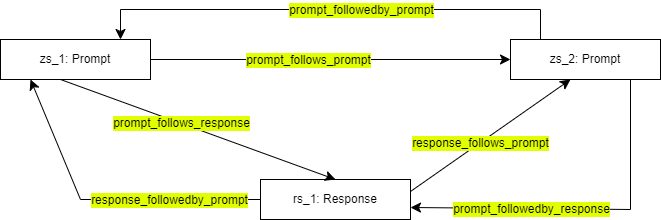
\includegraphics[width=0.9\linewidth]{Figures/fig_30.png}
    \caption{Chain prompt-response}
    \label{fig:enter-label}
\end{figure}
Of course, most of these relationships are automatically created during the inference process. To connect a response with the next prompt, we created this SWRL rule:
\begin{lstlisting}
peo:prompt_followedby_prompt(?x, ?y) ^ peo:prompt_follows_response(?y, ?r) -> peo:prompt_followedby_response(?x, ?r)
\end{lstlisting}
If a prompt $?x$ is followed by another prompt $?y$ and $?y$ has a response $?r$ then $?x$ is followed by $?r$. The context next prompt is assigned automatically using the object property \textit{prompt\_followedby\_prompt} ant this SWRL rule:
\begin{lstlisting}
peo:prompt_followedby_prompt(?x, ?y) ^ peo:has_context(?y, ?c) -> peo:has_context(?x, ?c)
\end{lstlisting}
If a prompt $x$ is followed by another prompt $y$ and $y$ has context the chat $c$ then $x$ has context $c$. Also each response is connected the chat using the object property \textit{is\_response\_of} (inverse property \textit{has\_response}) created using the SWRL rule:
\begin{lstlisting}
peo:response_followedby_prompt(?r, ?p) ^ peo:has_context(?p, ?c) -> peo:is_response_of(?r, ?c)
\end{lstlisting}
If a response $?r$ is followed by a prompt $?p$ and the prompt $?p$ has the context the chat $?c$ then the response $?r$ is response of $?c$. The last SWRL rule connects the response with the model that has generated it creating the object property \textit{response\_generated\_using} with inverse property \textit{generates\_response}:
\begin{lstlisting}
peo:response_followedby_prompt(?r, ?p) ^ peo:processed_by(?p, ?m) -> peo:response_generated_using(?r, ?m) 
\end{lstlisting}
If a response $?r$ is followed by a prompt $?p$ and the prompt $?p$ is processed by the LLM $?m$ then the response $?r$ is generated using $?m$.\\
All these object properties may seem unclear so below is a diagram that shows all the relationships involved in creating a chat.
\begin{figure}[H]
    \centering
    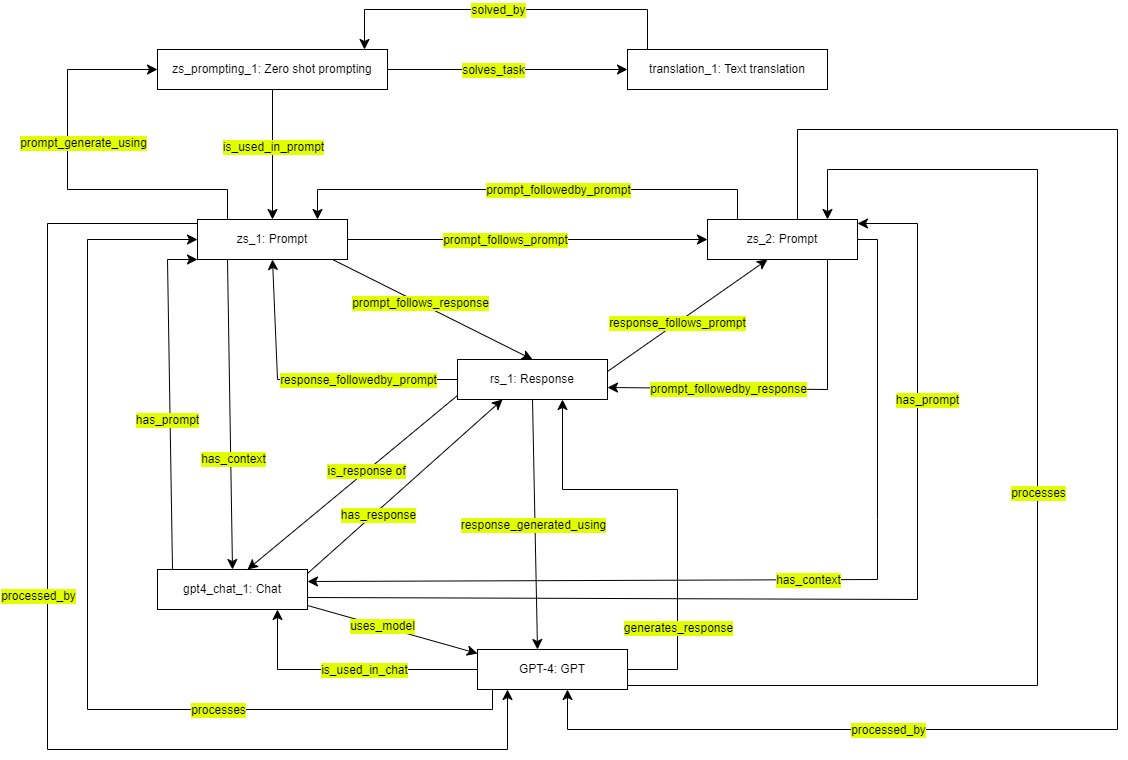
\includegraphics[width=0.85\linewidth]{Figures/fig_31.png}
    \caption{Chat scheme}
    \label{fig:enter-label}
\end{figure}


% \subsection{Ontology Population with prompts}
\subsection{Population with prompts}
\label{subsection:4_3_6_population}
Populating the ontology with prompts is a complex process as it requires connecting various instances (task, prompting technique, prompt, chat, response, LLM) using the defined object properties. Moreover, each prompt is manually crafted in accordance with the specific prompting technique. Manually populating the ontology with all instances for every task, every version of each LLM, and every prompting technique would be highly time-consuming and beyond the objectives of this thesis. Therefore, a decision was made to populate only a specific subset of the ontology choosing LLM versions, tasks and prompting techniques. Large language models chosed are very popular LLM available to the users and they are represented in the ontology:
\begin{itemize}
    \item \textbf{GPT-4}
    \item \textbf{Mistral-7B}
    \item \textbf{Gemini Flash}
\end{itemize}
Then I chosed five prompting techniques with a criterium for each one:
\begin{itemize}
    \item \textbf{Zero-shot prompting:} this technique allows LLMs to handle new tasks using only natural language instructions, without requiring examples or any effort by the user.

    \item \textbf{Few-shot prompting:} this technique  enables language models to learn new tasks with few examples, reducing the need for extensive task-specific datasets.
    
    \item \textbf{Role prompting:} this technique improves LLMs performance on solving tasks by simulating specific roles.

    \item \textbf{Emotion prompting:} this technique enhances LLMs by integrating emotions into prompts, improving response generation and performance on tasks.

    \item \textbf{Analogical prompting:} this technique is able to generate automatically task-specific exemplars, reducing manual annotation needs, and improving performance on problem-solving tasks.
\end{itemize}
Finally I chosed four task to solve applying prompting techniques and using LLMs defined:
\begin{itemize}
    \item \textbf{Emotion classification:} classification of the emotion in a given text.

    \item \textbf{Mathematical understanding:} solving a given mathematical problem of medium difficulty. 

    \item \textbf{Text translation:} translation of a text from english to italian.

    \item \textbf{Text summarization:} summarization of the content of a given text.
\end{itemize}
Below, we list the prompts created for each task.\\\\
\textbf{Task 1: Emotion classification}\\     
The text to classify the emotion is: \textit{"I think the vacation is okay"}
\begin{itemize}
    \item \textbf{Zero-shot prompting:} Classify the text into neutral, negative or positive. Text: "I think the vacation is okay." Sentiment:
    \item \textbf{Few-shot prompting:} Classify the following text into neutral, negative, or positive based on its sentiment. Here are some examples: 
    Text: "The food was absolutely wonderful!" Sentiment: Positive. 
    Text: "I did not enjoy the movie at all." Sentiment: Negative. 
    Text: "It was an average experience." Sentiment: Neutral. 
    Now, classify this text: Text: "I think the vacation is okay." Sentiment:
    \item \textbf{Emotion prompting:} Classify the following text into neutral, negative, or positive based on its sentiment. This task is very important to my career. Please provide a well-thought and accurate classification. Text: "I think the vacation is okay." Sentiment:
    \item \textbf{Role prompting:} From now on, you are an experienced sentiment analyst with deep expertise in understanding human emotions through textual analysis. Your task is to classify the sentiment of texts as neutral, negative, or positive with utmost accuracy and professionalism. Text: "I think the vacation is okay." Sentiment:
    \item \textbf{Analogical prompting:} Classify the text into neutral, negative or positive. \# Instruction: \# Text: I think the vacation is okay. \# Sentiment:
\end{itemize}
\textbf{Task 2: Mathematical understanding}\\
For the mathematical understanding there is the solving of a simple geometrical problem: the calculation of a square with the four vertices at (-2, 2), (2, -2), (-2, -6), and (-6, -2). 
\begin{itemize}
    \item \textbf{Zero-shot prompting:} What is the area of the square with the four vertices at $(-2, 2)$, $(2, -2)$, $(-2, -6)$, and $(-6, -2)$?
    \item \textbf{Few-shot prompting:} Instruction: Determine the area of a square given the coordinates of its four vertices. 
    Example 1: Vertices: $(0, 0)$, $(4, 0)$, $(4, 4)$, $(0, 4)$ 
    Step 1: Identify the side length. Distance between $(0, 0)$ and $(4, 0)$ is $\sqrt{((4 - 0)^2 + (0 - 0)^2)} = 4$. 
    Step 2: Calculate the area. Area = side length$^2 = 4^2 = 16$. Answer: 16. 
    Example 2: Vertices: $(-1, 1)$, $(-1, 3)$, $(1, 3)$, $(1, 1)$ 
    Step 1: Identify the side length. Distance between $(-1, 1)$ and $(-1, 3)$ is $\sqrt{((3 - 1)^2 + (1 - 1)^2)} = 2$. 
    Step 2: Calculate the area. Area = side length$^2 = 2^2 = 4$. Answer: 4. 
    Query: Vertices: $(-2, 2)$, $(2, -2)$, $(-2, -6)$, $(-6, -2)$. 
    Step 1: Identify the side length by calculating the distance between consecutive vertices. 
    Step 2: Calculate the area of the square. Answer:
    \item \textbf{Emotion prompting:} Please calculate the area of a square given the coordinates of its vertices. This task is important for building my understanding of geometry and improving my analytical skills, so I truly value a thorough and accurate solution. Vertices: $(-2, 2)$, $(2, -2)$, $(-2, -6)$, $(-6, -2)$.
    \item \textbf{Role prompting:} From now on, you are a brilliant geometry teacher. You always explain geometry problems thoroughly and ensure your students understand every step of the process. We have a question for you: I have four vertices of a square: $(-2, 2)$, $(2, -2)$, $(-2, -6)$, and $(-6, -2)$. Can you help me calculate the area of the square step by step? Please provide a detailed explanation of how to verify the shape, calculate the side length, and determine the area.
    \item \textbf{Analogical prompting:} What is the area of the square with the four vertices at $(-2, 2)$, $(2, -2)$, $(-2, -6)$, and $(-6, -2)$? \# Instruction: \#\# Recall relevant exemplars: \#\# Solve the initial problem:
\end{itemize}
\textbf{Task 3: Text translation}\\
For text translation task I chosed a citation of Lewis Carol \cite{carol} to translate form english to italian: \textit{"Sometimes, we've believed as many as six impossible things before breakfast."}
\begin{itemize}
    \item \textbf{Zero-shot prompting:} Translate the English text to Italian. Text: "Sometimes, we've believed as many as six impossible things before breakfast." Translation:
    \item \textbf{Few-shot prompting:} Translate the following English sentences into Italian: 
    1. English: "Sometimes, we've believed as many as six impossible things before breakfast." Italian: "A volte, ho creduto a ben sei cose impossibili prima di colazione." 
    2. English: "I think, therefore I am." Italian: "Penso, quindi sono." 
    3. English: "All the world's a stage, and all the men and women merely players." Italian: "Tutto il mondo è un palcoscenico e tutti gli uomini e le donne sono solo attori." 
    Now translate this sentence: English: "Sometimes, we've believed as many as six impossible things before breakfast." Italian:
    \item \textbf{Emotion prompting:} Translate the following text to Italian. It's very important for me to understand this translation accurately as it could affect my professional progress: "Sometimes, we've believed as many as six impossible things before breakfast."
    \item \textbf{Role prompting:} From now on, you are an excellent literary translation teacher who accurately explains the meaning and tone of complex sentences. Translate the following sentence from English to Italian, preserving its meaning and tone: "Sometimes, we've believed as many as six impossible things before breakfast."
    \item \textbf{Analogical prompting:} \# Problem: "Sometimes, we've believed as many as six impossible things before breakfast." 
    \# Relevant Problems: 
    1. Translating a complex sentence from English to Italian. 
    - Question: How to translate the sentence "To be or not to be, that is the question" into Italian? 
    - Answer: The sentence "To be or not to be, that is the question" translates into Italian as "Essere o non essere, questo è il problema." 
    2. Translating a sentence with idiomatic expressions. 
    - Question: How to translate "Break a leg!" into Italian? 
    - Answer: The idiomatic expression "Break a leg!" translates into Italian as "In bocca al lupo!" 
    3. Translating a sentence with abstract concepts. 
    - Question: How to translate "The only limit is your imagination" into Italian? 
    - Answer: The sentence "The only limit is your imagination" translates into Italian as "L'unico limite è la tua immaginazione." 
    \# Translation of the initial problem: The sentence "Sometimes, we've believed as many as six impossible things before breakfast" translates into Italian as:
\end{itemize}
\textbf{Task 4: Text summarization}\\
The last task is the summarization of the following text about permaculture: \textit{"Permaculture is a design process mimicking the diversity, functionality and resilience of natural ecosystems. The principles and practices are drawn from traditional ecological knowledge of indigenous cultures combined with modern scientific understanding and technological innovations. Permaculture design provides a framework helping individuals and communities develop innovative, creative and effective strategies for meeting basic needs while preparing for and mitigating the projected impacts of climate change."}\cite{permaculture}
\begin{itemize}
    \item \textbf{Zero-shot prompting:} Permaculture is a design process mimicking the diversity, functionality and resilience of natural ecosystems. The principles and practices are drawn from traditional ecological knowledge of indigenous cultures combined with modern scientific understanding and technological innovations. Permaculture design provides a framework helping individuals and communities develop innovative, creative and effective strategies for meeting basic needs while preparing for and mitigating the projected impacts of climate change. Write a summary of the above text. Summary:
    \item \textbf{Few-shot prompting:} You are an expert at creating concise summaries. Below are some examples of summaries based on texts.
    Example 1: Text: The Earth orbits the Sun in an elliptical pattern, taking approximately 365.25 days to complete one orbit. This forms the basis of the Gregorian calendar year. Summary: The Earth completes an orbit around the Sun in roughly 365 days, defining the calendar year.
    Example 2: Text: Sustainable agriculture incorporates practices that maintain productivity and minimize environmental impact, such as crop rotation and organic farming. Summary: Sustainable agriculture uses eco-friendly practices like crop rotation and organic methods to maintain productivity.
    Task: Text: Permaculture is a design process mimicking the diversity, functionality, and resilience of natural ecosystems. The principles and practices are drawn from traditional ecological knowledge of indigenous cultures combined with modern scientific understanding and technological innovations. Permaculture design provides a framework helping individuals and communities develop innovative, creative, and effective strategies for meeting basic needs while preparing for and mitigating the projected impacts of climate change. Summary:
    \item \textbf{Emotion prompting:} Summarize the essence of permaculture, focusing on its innovative design process inspired by natural ecosystems. Highlight how it combines traditional ecological knowledge with modern science and technology to address climate change. This understanding is vital to my research and the future of sustainable living. Please ensure the summary is concise yet comprehensive.
    \item \textbf{Role prompting:} From now on, you are an environmental scientist who specializes in explaining complex ecological concepts in an accessible and engaging manner. Your task is to provide a concise summary of permaculture principles and their importance in addressing climate challenges.
    \item \textbf{Analogical prompting:} Problem: Summarize the definition and essence of permaculture using principles that mirror natural ecosystems and combine traditional ecological knowledge with modern science. Instruction: Recall three relevant and distinct problems or topics related to summarizing processes that focus on mimicking complex systems. Provide detailed exemplars for each recalled instance, including how the principles were extracted and utilized effectively. Use the recalled insights to structure and write the final summary.
\end{itemize}
The responses for each prompt from the three LLMs have been saved in the ontology, and a chat has been created for each prompt, including a title, start time, and end time resulting in a total of 60 distinct chats.
\begin{figure}[H]
    \centering
    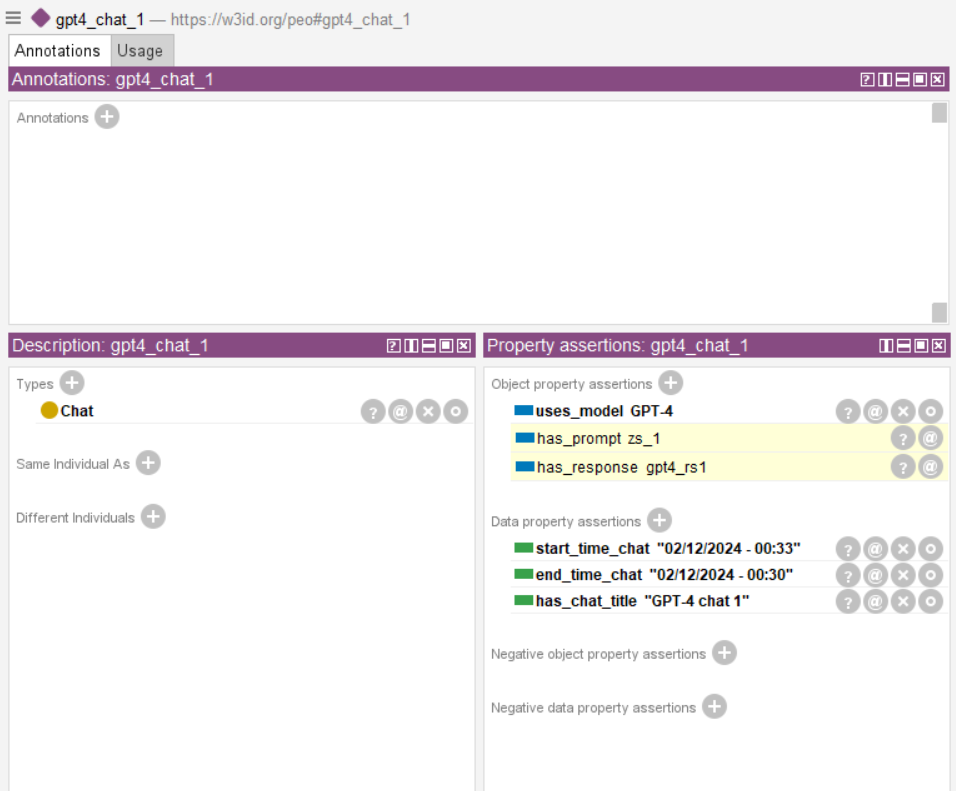
\includegraphics[width=0.75\linewidth]{Figures/fig_32.png}
    \caption{Example of chat with relations inferred}
    \label{fig:enter-label}
\end{figure}

% \subsection{Automatic ontology population}
\subsection{Automatic Population}
\label{subsection:4_3_7_automatic}
Populating an ontology with various instances can be a time-consuming task for developers, as the ontology's domain of interest often involves numerous entities requiring manual insertion. To streamline this process and reduce the developer's effort, automation can be employed. There are different researches dedicated to the automatic population of ontologies, one of the most recent is \textit{"Ontology Population using LLMs"} \cite{norouzi2024ontology}, it proposes a methodology to semi-automatically populate modular ontologies using Large Language Models (LLMs). It focuses on leveraging the strengths of LLMs, such as GPT-4 and Llama-3, for extracting structured knowledge from natural language texts. The method is divided into three main stages: data preprocessing, relevant text retrieval, and ontology population. In the first stage, the data is cleaned, organized, and aligned with simplified ontology modules to facilitate processing. The second stage employs text summarization and Retrieval-Augmented Generation (RAG) techniques to identify and extract relevant information aligned with the ontology schema. Finally, in the third stage, predefined module files guide the LLMs to populate the ontology with accurate triples by using structured prompts. Despite the good results, the methodology still requires effort, as documents need to be selected and preprocessed to create a dataset that serves as input for the LLM used to populate the ontology. Implementing this process demands skills that go beyond those of an ontology engineer, effectively shifting the workload to another task.\\ 
Another approach is proposed in the paper \textit{"Financial Product Ontology Population with Large Language Models"} \cite{saetia2024financial}, it leverages Large Language Models (LLMs), such as GPT-3.5 and GPT-4, to populate financial ontologies by extracting structured data from unstructured texts. It combines several prompting techniques to improve accuracy and scalability. Few-shot prompting provides positive and negative examples to guide the model's understanding. Chain-of-Thought (CoT) reasoning encourages sequential reasoning, while schema.org definitions are included to contextualize fields and properties. Prompts are carefully designed to generate structured outputs in JSON format for easy integration and evaluating performance using F1 scores, with the best results achieved when combining examples, CoT, and definitions. Like the previous one, this approach requires a lot of job on gathering necessary docs to pre-process and this process can be time-consuming, also the quality of the output depends on the prompts.\\ These tasks divert attention from the main objective and increase the developer's workload. Rather than using the methodologies outlined in the literature, we opted for a more straightforward and pragmatic approach to populating the ontology. Starting from the sixteen competency questions defined in the \textit{Ontology requirements specification} section, we input them, together with the ontology, into a LLM to generate an automatically populated version of the prompt engineering ontology. The LLM chosed is GPT-4o: the latest and most powerful version of GPT available in its web interface ChatGPT \footnote{https://chatgpt.com/} and used previously in the manual ontology population. This time instead of giving as input a specific prompt created with one of prompt engineering techniques, we write this prompt, providing the ontology and a text file containing the competency questions.
\begin{figure}[H]
    \centering
    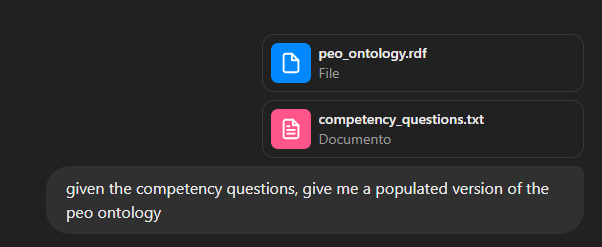
\includegraphics[width=0.9\linewidth]{Figures/fig_34.png}
    \caption{Prompt for automatic ontology population}
    \label{fig:34}
\end{figure}
After this prompt the LLM begins a reasoning process, first it explains the approach followed by the model:
\begin{figure}[H]
    \centering
    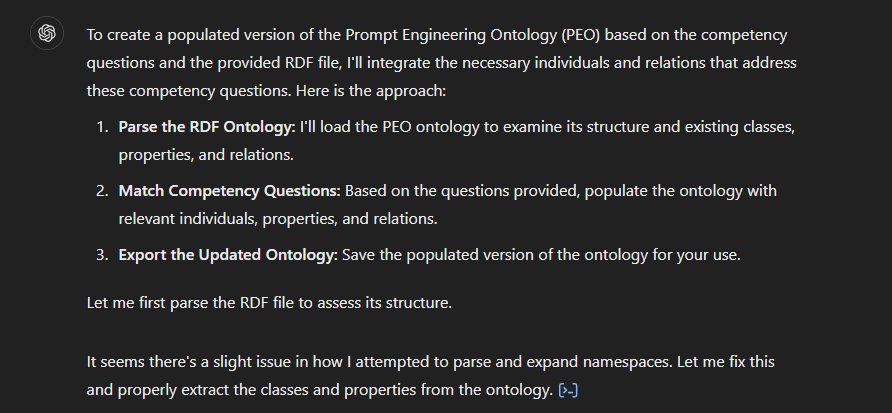
\includegraphics[width=0.9\linewidth]{Figures/fig_35.png}
    \caption{First GPT-4 output in the automatic population}
    \label{fig:enter-label}
\end{figure}
Then the model analyses the ontology structure encoded in the RDF file, listing simple classes and sample object properties found:
\begin{figure}[H]
    \centering
    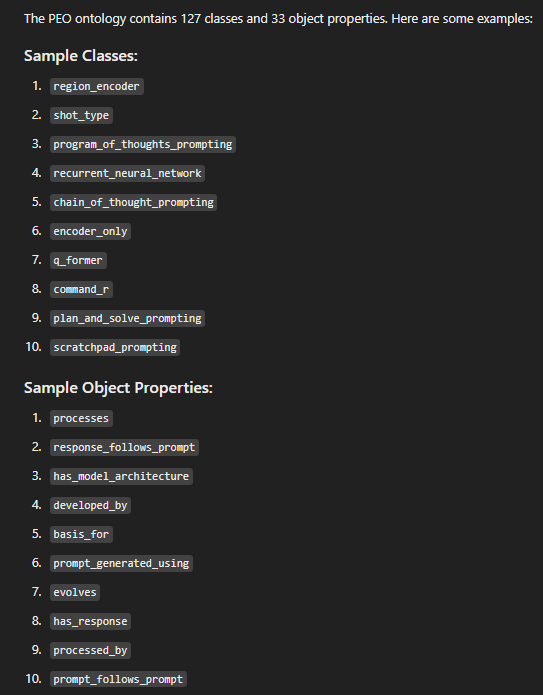
\includegraphics[width=0.85\linewidth]{Figures/fig_36.png}
    \caption{Structure analysis of the ontology}
    \label{fig:enter-label}
\end{figure}
Finally it produces the downloadable RDF file containing the ontology populated by the model:
\begin{figure}[H]
    \centering
    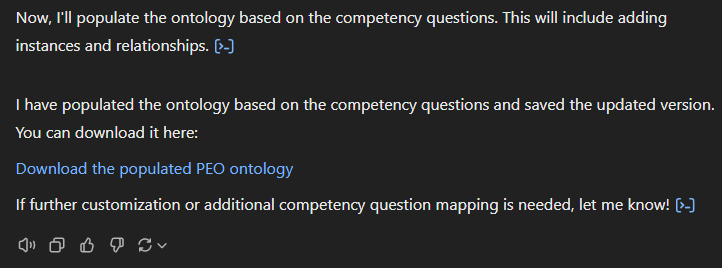
\includegraphics[width=0.9\linewidth]{Figures/fig_37.png}
    \caption{Final LLM output}
    \label{fig:enter-label}
\end{figure}
After downloading the RDF file, we open it using the Protegé editor to see the final result. At a first glance, the obtained result seems rather poor, as four new classes have been created again without considering the classes already present in the ontology:
\begin{itemize}
    \item \textbf{PromptEngineering}
    \item \textbf{Prompt}
    \item \textbf{PromptingTechnique}
    \item \textbf{Task}
\end{itemize}
without considering the hierarchy defined in the ontology as we can see:
\begin{figure}[H]
    \centering
    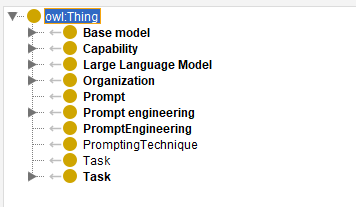
\includegraphics[width=0.9\linewidth]{Figures/fig_38.png}
    \caption{PEO populated automatically}
    \label{fig:enter-label}
\end{figure}
Just two classes have a definition: Prompt and PromptEngineering with no individuals created while the PromptingTechnique class has no defintion and three individuals created:
\begin{itemize}
    \item ChainOfThoughtPrompting
    \item FewShotPrompting
    \item ZeroShotPrompting
\end{itemize}
There is no new instance of chat and all the mechanism defined to link a prompting technique with a chat is completely ignored. No new object properties or data properties have been created by GPT-4o, just an annotation property called \textit{hasDefinition}. Any other useful information is not created, the three entities are not linked with any object property and they do not have any data property. Additional prompts would clearly be needed as input for the LLM to improve the result, which is currently poor and adds no useful information compared to the original, manually populated version of the prompt engineering ontology.